\section{Literature Review}
This section will investigate the current state of the scientific knowledge 
about the relevant topics of this thesis. The first section will explain 
what the current state of object detection on embedded devices is.
This is then followed by discussing how the problem 
of controlling the drone using RL has been solved in earlier studies and how 
this thesis will aim at optimizing this process. Finally, 
as has been mentioned before, the RL algorithm will be trained in a simulation 
environment. Deploying such an agent to the real-world brings with it a set of 
problems that will be addressed.

\subsection{Object Detection}
The primary problem to solve is to make sure 
that the drone is able to detect the required object to follow. This problem is 
most effectively solved by the use of neural network models that have been specifically 
trained to detect a vast variety of objects. The attempts at solving the object 
detection problem using neural networks has already been a topic of interest for 
more than a decade \cite{original-rcnn}. The first largest breakthrough in this area 
has been the application of a combination of networks \cite{original-rcnn}. 
The first part of this combination is a Convolutional Neural Network (CNN), which is a model that 
performs object classification by extracting low-level 
spatial features from the images and combining these into high-level features before 
classifying the image into a set of classes. The second part is a region proposal 
network which propose regions 
where objects could be present. By having the first part of the network perform region proposals, 
and supplying these to a CNN, the R-CNN network was significantly able to increase speed and
accuracy in object detection models. Nonetheless, this network was soon improved by performing the 
input to the CNN in one forward sweep for all the different proposed regions in the 
previous step \cite{fastrcnn}. Finally, combining the whole process, provided the final 
step in accurate and reliable object detection \cite{fasterrcnn}. 

However, these improvements, although vastly progressing the speed and accuracy of the 
models, have still left room for networks that might sacrifice a proportion of accuracy 
for the sake of speed. The most notable model that has been able to do this, is called 
You Only Look Once (YOLO) \cite{originalyolo}. The idea is to only perform a single pass 
through a network per image, and get the required predictions. This is done by first 
dividing the image into an $S \times S$ grid. For each of these grid cells, the model 
predicts $N$ amount of bounding boxes and corresponding confidence scores. These 
bounding boxes are possible rectangles that enclose an object. Then, for each of these 
bounding boxes, a probability distribution over the possible classes is performed. 
From this set of bounding boxes with corresponding class probabilities, the bounding 
boxes with the highest confidences are preserved, leaving a set of bounding boxes and 
their corresponding class predictions for each object behind. Performing object detection 
using this technique vastly improves the speed while only minimally sacrificing accuracy.
Additionally, through the use of neural network optimization techniques, this model has 
seen drastic improvements in later years as new versions of it have been introduced \cite{yolo9000,yolov3, YOLOv4}.
These YOLO algorithms deliver much higher speeds while minimally sacrificing accuracies. 
Situations such as embedded devices could use these aspects of these object detectors. 

However, alongside with the increase in research into these 
YOLO algorithms, there has also been research into developing these models for 
low computational devices \cite{YOLO-Lite,Mixed-Yolo_Lite, yolov3-tiny}. 
The method that has been used in these to reduce the computational load have been 
either pruning methods, where parameters least crucial to the final output are discarded,
or by creating a similar network architecture with less parameters and performing the training process anew. 
Nonetheless, they still sacrifice a 
significant proportion of accuracy for the sake of speed on EDs. 


\subsubsection{Human Detection}
As a subset of Object Detection, human detection has been a field that has benefited
greatly from the advances in Deep Learning (DL). From the first large breakthroughs of 
the field \cite{haarcascades, HOGdetection} the contribution of DL is still not 
outperformed. Problems such as trouble finding humans in different poses and unreliable 
bounding boxes make the alternative much more attractive. Using DL networks for the 
object detection problem has been able to perform the task without these problems. This 
leaves the use of the previously described object detectors, as the best option in order 
to perform overall human detection in most cases where the previously discussed issues 
are vital. 

\subsection{Reinforcement Learning}
The method of performing obstacle avoidance and following in this thesis
is to use Reinforcement Learning (RL). RL is a type of Machine Learning that 
focuses on mapping situations to actions according to the maximization of a 
numerical reward function \cite{RLBook}. The main process of learning here is to 
adapt a decision maker, which we will call an agent, according to experiences \cite{rainbowrl}. 
Here an attempt is made to perform the action, after which a reward is given in 
the form of a scalar value by the environment, which are all the externalities 
that determine what state the agent is in. This reward is then used as a cue  
to alter the mapping from states to actions accordingly. This process allows 
the agent to learn from experience on how to act in order to achieve the desired 
behavior. The foundation of RL is based on the collaboration between the agent 
and the environment. For each time step, the agent 
finds itself in a certain state. During this state, the agent has a certain set 
of actions that it can choose from. For each of these actions, there 
is an effect on the environment. Therefore, the agent finds itself 
in a new state, repeating the process of action-selection. This process is 
illustrated in Figure \ref{AgentEnv}. 

\begin{Figure}
    \centering
    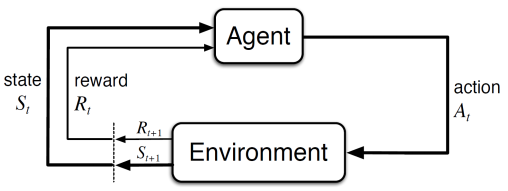
\includegraphics[width=\linewidth]{AgentEnv.png}
    \captionof{figure}{Agent-Environment interaction in RL}
    \label{AgentEnv}
\end{Figure}

The essence of this algorithm is based on the environment's response to each 
action that the agent chooses. The environment, during training time, gives 
the agent either a reward (possibly in the form of punishment) that the agent 
uses to gather experiences. This reward is based on a function which 
determines what the agent will try to optimize and therefore by definition, what the 
agent will try to learn. 

Formally, this process takes an arbitrarily defined timestep $t$, and provides
the agent with a state $S_t$. Given this state $S_t$, the agent decides on 
an action $a$ out of the possible available actions $A$ using a certain policy $\pi$.
Performing this action changes the environment and provides the agent with a 
new state: $S_{t+1}$. Together with this new state, the environment also 
provides the agent with a reward $r_{t+1}$. The eventual learning goal of the agent,
is to find a policy $a = \pi(s)$ that maximizes the overall reward that he will
receive. This requires taking into account future rewards as well, which is 
recorded in the return $R_t$ of a certain action in a specific state. 
However, what actions will be chosen by the agent is dependent on the policy $\pi$
that the agent employs. The policy is defined as a probability distribution over
the possible actions for each state. The goal is therefore to maximize its 
return by defining a certain policy. 

An important concept here is the balance between exploration and exploitation. 
When the policy is completely directed towards exploitation, the agent will 
not explore many of the other possible actions that can be taken that could 
potentially lead to higher returns. However, if an agent is fully committed to 
exploration, it will never maximize the returns and will keep exploring the space 
without settling on any maxima. The policy which perform the best are therefore, 
the ones that are able to balance both of these strategies in order to maximize 
the overall returns. 

\subsubsection{Q-Learning}
There are multiple ways in which to approach the learning problem in RL. 
One of these is to focus on the determination of the $Q$-values. These values
connect the action with the states and ascribe to them a value. This value
represents the expected return for choosing an action $a$ in state $s$, 
expressed as $Q(s, a)=\mathbb{E}_{\pi}\left[R_{t} \mid s_{t}=s, a_{t}=a\right]$.
Intuitively, the expected return is the total sum of expected reward that will be 
collected by choosing this action and continuing from there onwards. This leads to 
the following simplified equation:

\begin{equation}
    Q(s, a)=r+\gamma \max_{a^{\prime}} Q\left(s^{\prime}, a^{\prime}\right)
\end{equation}

The function of this equation is, therefore, to update the $Q$-values throughout
the learning process. Since these values represent the overall return of choosing
an action, this will create a mapping from each state to what the value is of each action in a state,
taking into account later states. Having this information provides the algorithm 
with an overview of what action to take in each situation by choosing the action with the 
highest $Q$-value for that specific state. 

\subsubsection{Deep Q-Network}
In the domain of this thesis the actions 
that the RL algorithm can choose from are a discrete set that consist of directions 
that the drone can go towards. The states, however, are a continuous space that are 
represented by the bounding box of its target on the input image and an additional image, 
either depth- or normal-image. 

Keeping a tabular representation of the mapping of 
each state to its possible actions would vastly inflate the amount of information 
that the algorithm would need to keep track of. This means that there is a necessity 
to represent the action space, not categorically, but as a function. 

This is where 
the previously described neural network approach comes into play. Deep CNNs are 
used in order to do the mapping of a continuous state to a discrete action space \cite{DQNDeepmind}. 
The DQN chooses its actions using a $\epsilon$-greedy policy, which is to say the 
action with the highest $Q$-value is chosen, except for a $\epsilon$ proportion 
of the time where another action is chosen randomly. 

For each of these timesteps 
the DQN stores the experience, which is a sequence of $(S_t, A_t, R_{t+1}, S_{t+1})$, 
to a replay memory buffer. This buffer tracks a million of the most recent experiences 
of the agent. Using this buffer, a random sample of experiences are taken and 
fed forward through the CNN, adjusting its mapping from states to actions. This 
has been developed for smoother learning as the agent refers back to a larger memory of 
experiences throughout the learning process and is not as prone to variations 
in parameters. 

\subsubsection{Reward function}
It becomes apparent that the most crucial aspect of what the agent will learn 
is mostly dependent on the reward function that determines what reward the 
RL algorithm will receive throughout each time-step. The definition of a reward 
function therefore becomes crucial in the process of training an agent with a 
behavioral goal in mind. The engineering of a reward function can therefore be 
approached differently. 

The easiest way in which to do this is to simply mark 
the states where the goal has been achieved and mark the remainder of the states 
as being failed. This formalizes what states the agent will trying to achieve 
very clearly. However, this also brings with it some complications during the 
learning process as this means that the agent will be exploring a vast amount 
of state-space where no reward signal is given. 

On the other hand, the state-space can also be given a certain type of reward 
function that reflects an ordering of the states in a way that represents how close 
an agent is to the goal state. However, the disadvantages here are that this 
requires domain-specific knowledge about when an agent is closer to the goal or not. 
This imbuing of some predetermined knowledge in the reward function also blocks 
the agent from finding new ways to solve the problem. Performing 
this reward function engineering is also a limitation in situations where the 
composition of permissible behavior is not know prior to training \cite{rewardshaping}. 

This makes the alternative of having a delimited goal space much more attractive, 
even when considering the sparse rewards that it might give. 

\subsubsection{Hindsight Experience Replay}
Domains with sparse rewards pose some challenges in the training process. Since 
many of the states possess rewards that are negative, there are not many instances 
of experiences where the agent receives a reward signal that is significant for it 
to relate what it would need to do to maximize this reward signal. In the domain of 
the drone operating in the simulation, only in the camera shots where the drone is actually 
including a person, is there a positive reward. It therefore become extremely 
difficult for the RL algorithm to learn in this environment, because the instances 
where it does receive a reward are very sparse. 

A large breakthrough in 
training RL agents in sparse reward environments has been the concept of 
Hindsight Experience Replay (HER). Closely related to the experience buffer that 
has been mentioned, this method uses previous experiences that have not performed 
the task successfully, and reshapes them into positive experiences. By taking a 
sample from the experience replay buffer, and changing the received reward for 
that experience to a positive reward, as if the goal had been reached in that state, 
the experience can be used as though it had been a successful attempt at performing 
the task. This simple method, has provided many robotic applications with a faster 
learning curve and better performance \cite{HER}. 

However, the application of HER in the domain of a drone operating in a virtual 
environment has not been performed before. Many of the applications have included 
simulated environments where a robotics task is being performed. The 
behaviors that HER significantly improved have been tasks where a sequential 
approach to solving the problem was necessary. In the case of the drone, there 
is a similar requirement where the drone would need to perform a sequence of tasks 
in order for the target person to be visible in its view. The application of 
the HER method could lend itself very well to the domain of the drone following 
task. 

\subsection{Obstacle Detection Technologies}
Next to the target to be followed, another problem is the obstacle avoidance issue. 
The problem here is that the agent requires some type of information in its input 
to be able to deduce whether an obstacle is in its way. Therefore, the primary problem to solve is what sensory 
information the agent has access to, to be able to determine whether obstacles are present. 
Many attempts have implemented deep neural networks to perform 
the object detection, and included additional hardware to perform the obstacle detection \cite{Visual-GPS, lidarinselfdrivingcar,acousticdronefollower}.  
More remarkably, there is an increasing interest in performing the obstacle avoidance 
task using only computer vision techniques. Both of these will be explored. 

\subsubsection{Additional hardware}
Many solutions to the problem of obstacle avoidance have been to install a 
certain type of sensor technology in order to detect obstacles. Technologies such as 
LiDAR \cite{ObstacleAvoidance}, for example, are being used in many devices that require 
the ability to potentially avoid objects in order to follow a certain path. A most notable
example of this application has been in self-driving cars \cite{lidarinselfdrivingcar}. LiDAR 
works by emitting strobes of light at the scene and recording the return time of these 
strobes. This can be used to sense the distance from the objects in around the sensor. 
Next to this, the use of acoustic signals as a way of detecting obstacles has been used 
in the case of flying unmanned drones \cite{acousticdronefollower}. This is similar to the 
LiDAR technology but instead uses sonar waves to calculate the distances of the objects 
around the object. However, a considerable disadvantage of these types of sensors are that 
both of them add a physical weight to the device which impedes the movement of 
the drone, posing a limitation to the use of these techniques. The preference would still 
go towards a method that would omit the need for extra hardware. 

\subsubsection{Depth Perception}
At the same time, another technology to use for obstacle avoidance is to 
solely rely on the camera to perform the task. This allows the 
system to detect and avoid possible obstacles in its path without the need for 
extra hardware to perform this detection. When it comes to the limited resources of an ED, the preference 
goes to these methods.

One of these vision-based methods for obstacles detection is depth-perception.
The use of depth-perception greatly reduces the necessity of the drone to recognize 
other objects next to the target object. This technology works by using two
cameras that are setup to take an image simultaneously. By finding the pixel that 
corresponds to the pixel in the other image taken, the disparity between both of 
these pixels can be used to calculate the distance of the two cameras to that point.

Similarly to humans, this would allow the drone to recognize that something is in its way, 
without the necessity to recognize what it is that is obstructing its path. Using a 
depth perception image as an input for any decision making process could vastly simplify 
the problem of obstacle avoidance all together. 
Using depth-images as an input to a RL algorithm has been performed before \cite{iowamasterthesis},
however, whether this improved the performance compared to direct camera input or 
whether this translated to real-world applications is still missing. Testing whether 
the depth-perception adds an easier training process and whether it allows for generalization 
to real-world applications is therefore still relevant and a interesting option to use 
as an input to a RL agent. 

Many of the depth-imaging technologies face difficulties performing accurate 
depth perception in various circumstances. This is especially the case when the required distance becomes 
larger than a couple of meters \cite{stereovision}. However, since the application 
of this thesis is to let the drone perform indoor environments, this limitation 
becomes less relevant, especially considering that stereo vision is capable of performing
depth-imaging within 2 meters with a maximum error margin of 10\%. 

\subsection{Embedded Device}
This thesis will focus on the implementation
of these algorithms on an embedded devices (EDs). These devices are per definition poor in 
computational resources because they are developed with a specific functionality 
in mind \cite{embeddedsystem}. Therefore, the aforementioned problems of physical and 
computational limitations are . Indoor drones are modest in size and consequently, 
also in computing power. There are certain approaches that can be used in order to 
circumvent or solve this problem of lower computation. These include cloud computing or
a ground controller \cite{cloudcomputingdrone, ParrotARDrone}. However, these also 
pose limitations to the flying range, capabilities and add latency that only 
increase the list of constraints to the computationally limited drone. 

The focus in this thesis is therefore to keep the necessary algorithms  
computationally low. This would come with additional 
efforts into creating smaller or computationally lighter algorithms without
drastic loss in functionality. The previously mentioned pruning techniques that 
the object detectors have used to develop lighter and faster versions are relevant 
for devices such as these. The reduction in computational power that these methods 
require leaves more room for the DQN. 
